\documentclass[10pt]{article}
\usepackage[a4paper,bottom=3cm]{geometry}
\usepackage[english]{babel}
\usepackage[utf8]{inputenc}
\usepackage{amsmath}
\usepackage{amssymb}
\usepackage{graphicx}
\usepackage{subfig}
\usepackage{hyperref}

\author{Takudzwa Togarepi, Julian Bopp }
\title{Project Part 1: Probabilistic modeling of the femur anatomy}
\begin{document}

\maketitle
\begin{abstract}
    Describe the project in a few sentences. 
    The reader should get an idea of what the project is all about
    and what you achieved in the project.


    In this first part of the project ''Sex and stature prediction from partial femurs using statistical shape modelling'' we build,
    analyze and validate a model of the femur shape.
\end{abstract}

\section{Introduction}

We build, analyze and validate a model of the femur anatomy. Probabilistic modeling of femur anatomy has important applications in medical imaging, including computer-assisted surgery, patient-specific implant design, and bone fracture analysis. By accurate modeling of anatomical landmarks on the femur, these techniques can help improve surgical outcomes and reduce complications. In particular we construct a Gaussian Process (GP) Model using a dataset consisting of data from 46 femurs.
\section{Methods}

In this section you can describe the methods you used to solve the problem.

\newpage
\section{Experiments and results}
\subsection{Data and experimental setup}

%Explain the data with which you are experimenting.
%Highlight aspects of the data that are particularly interesting
%for the project.

The data on which we are experimenting consists of 46 femurs. Included in this data are landmarks $L0,\dots,L5$ for every femur.
In particular $L3,L4$, as seen in figure \ref{fig:landmark_width}, can be used to estimate the width of the femur, whereas $L2,L5$, as seen in figure \ref{fig:landmark_length}, can be used to estimate the length.

\begin{figure}[h]
\centering
\includegraphics[scale=0.2]{screenshots/L3blue_L4red_width.png}
\caption{Landmark $L3$ in blue, and landmark $L4$ in red. Used to estimate width of the femur bone.}
\label{fig:landmark_width}
\end{figure}

\begin{figure}[h]
\centering
\includegraphics[scale=0.2]{screenshots/L2red_L5green_length.png}
\caption{Landmark $L3$ in blue, and landmark $L4$ in red. Used to estimate length of the femur bone.}
\label{fig:landmark_length}
\end{figure}
\noindent
To estimate the length of a femur we calculate the distance between the $L2$ and $L5$ landmark, similarliy we estimate the width by calculating the distance between the $L3$ and $L4$ landmark. We display the measurements made from the 46 femurs in figure \ref{fig:scatterplot_femurdata} and summarize them in table \ref{table:mean_variance_femur_data} by calculating the mean and variance.
\begin{figure}
\centering
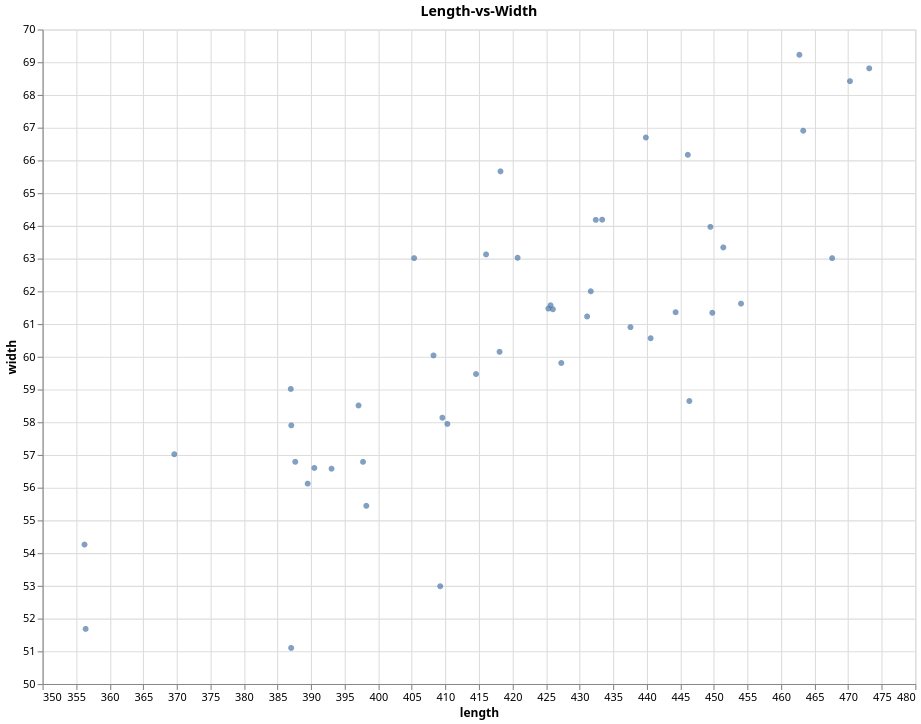
\includegraphics[scale=0.4]{screenshots/femur_data_length_width_scatter.png}
\caption{Scatterplot of calculated length and width of the femur data}
\label{fig:scatterplot_femurdata}
\end{figure}

\begin{table}[h!]
\centering
\begin{tabular}{c|r|r}
 & Mean & Variance \\
\hline
Length & 420.80 & 841.94 \\
Width & 60.61 & 18.13
\end{tabular}
\caption{Mean and variance of length and width of the femur data.}
\label{table:mean_variance_femur_data}
\end{table}

\noindent
We notice a high variability of the data. This gives reason to believe that the 46 femur samples are not from subjects that all share similar height attributes. More precisely, the data probabably originates from males and females with a large variability in height, and therefore, a large variability in femur length and width. Visually, figure \ref{fig:scatterplot_femurdata} gives reason to believe that the length and width are correlated. There is a trend that shows that an increase in length comes with an increase in width.




% Side by Side picture mode
%\begin{figure}%
%    \centering
%    \subfloat[\centering label 1]{{\includegraphics[width=5cm]{../screenshots/L3blue_L4red_width.png} }}%
%    \qquad
%    \subfloat[\centering label 2]{{\includegraphics[width=5cm]{../screenshots/L2red_L5green_length.png} }}%
%    \caption{2 Figures side by side}%
%    \label{fig:example}%
%\end{figure}

\newpage
\subsection{Experimental results}

\newpage
\section{Conclusion}

Add your conclusion here. What is the main result? What did you achieve, what 
needs to be done. 


\end{document}
